%Chapter of Design

\chapter{Design}
\label{design}

\section{Aims}

The basic aims are to design and implement a basic protocol for the transmission data to a server. This protocol will have security such that the messages are protected from modification, spoofing and can't be read in transit. There is to be a server application that allows the user to view the data being sent to the server.
Following on, the needs of machine to machine communication will be considered and the protocol will be expanded to include direct communication and secure transmission of keys. Finally, as this will be on a low powered device, the power usage is to be measured to establish performance and power overhead of security. 

``prevents rogue devices from transmitting data to others''?!?!

\section{Microcontroller}

The first step in this application is the acquisition of data. For example data, a variable that is monitored for important applications in the real world was chosen, this being temperature. There are a range of temperature sensors out there but one that is compact, cheap, freely available, has a large temperature range, high precision and can derive power directly form the data line, so called parasite power, is the DS18S20. It returns a 9-bit byte array so is ready to encrypt straight away. 

\begin{figure}[h]
	\centering
	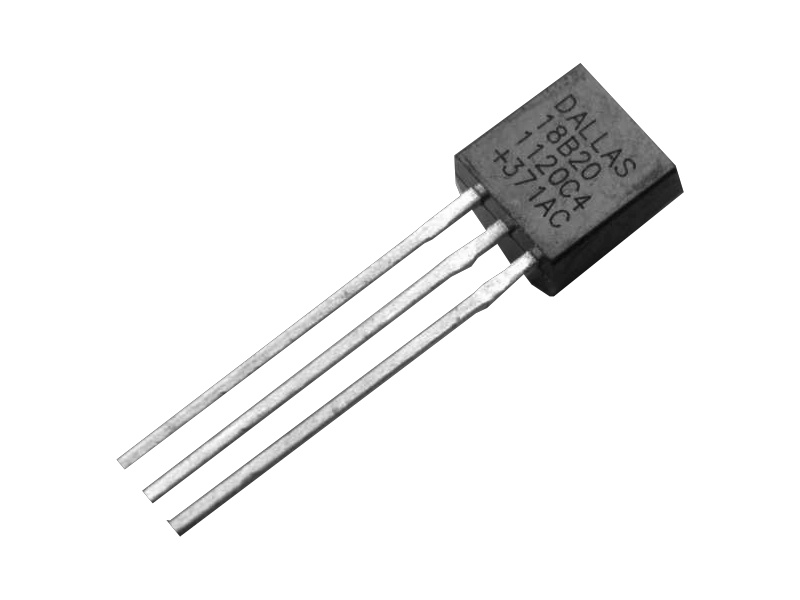
\includegraphics[width=.4\linewidth]{Figures/ds.jpg}
	\caption{DS18S20 Temperature Sensor}
	\label{fig:ds}
\end{figure}

The Arduino Due is a large Arduino, it is the first one with a 32-bit ARM core micrcontroller, has 54 digital I/O pins, 512KB flash memory, 96KB SRAM and a 84MHz. 
A lot of microcontrollers are 8-bit which means that they are limited in their cryptographic options. With a 32-BIT architecture and a large amount of flash memory it is possible to have a light weight cryptographic library for our application but the Due is still low cost enough that it can be used for an IoT sensor application. Because it is an Arduino it benefits from the large community, wide range of compatible components and large set of open source libraries.

\begin{figure}[h]
	\centering
	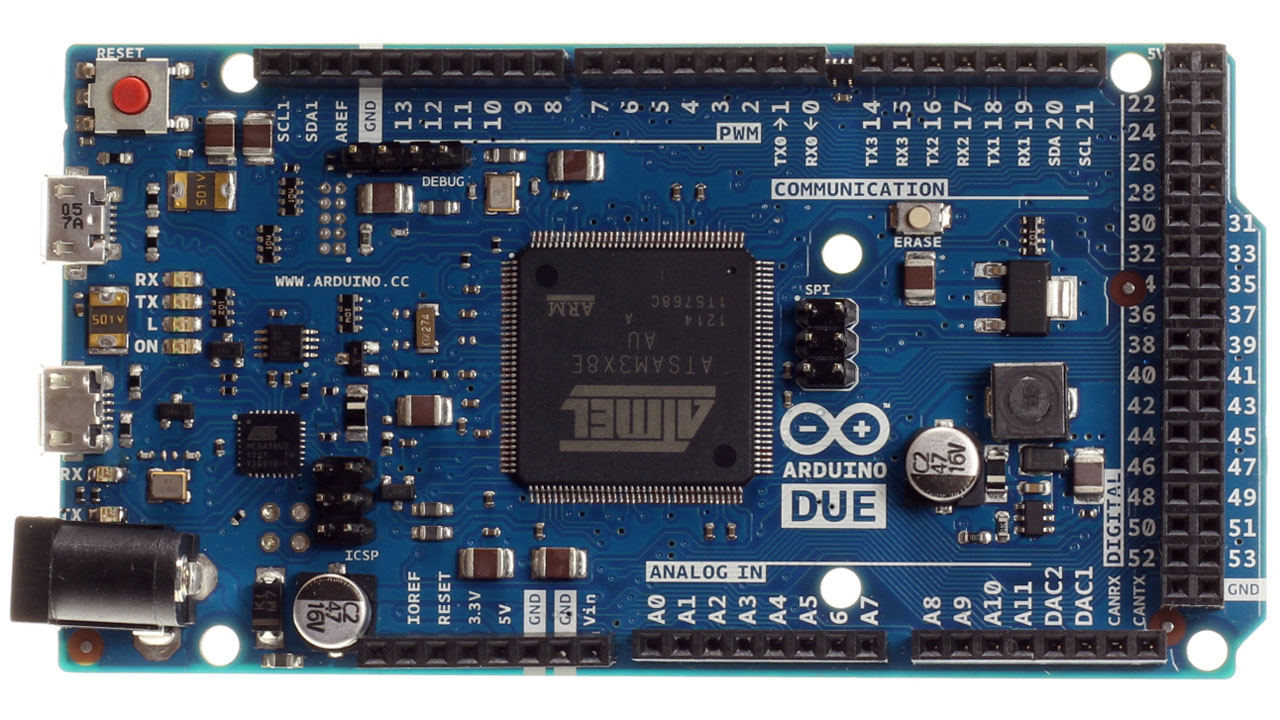
\includegraphics[width=.4\linewidth]{Figures/due.jpg}
	\caption{DS18S20 Temperature Sensor}
	\label{fig:ds}
\end{figure}

Once the temperature data is on the board there needs to be a way to transmit the data, as the data is being sent over the internet the natural choice is an Ethernet or WiFi shield. Unfortunately although the WiFi shield would be better, as wireless improves and becomes more the norm, the more IoT applications will use it, it is much more expensive than the Ethernet Shield. The first revision of the shield is no longer made so the second revision, R2 will be utilised. IT allows for easy connection for the Arduino to the Internet, it uses the Wiznet W5500 Ethernet chip, supports up to 8 different socket connections at a speed of 10/100Mb and has a MicroSD card slot to store network settings. 

\begin{figure}[h]
	\centering
	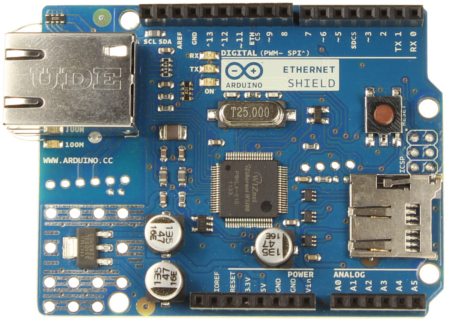
\includegraphics[width=.4\linewidth]{Figures/ethernet.jpg}
	\caption{DS18S20 Temperature Sensor}
	\label{fig:ds}
\end{figure}

\section{Security}

There a lot of security options for desktop programmes and communications like AES, WEP, SSL. In this more ubiquitous field the implementations have been around for a while but for microcontrollers only in recent times have they become powerful enough at a cheap price and therefore popular enough for developers to write or adapt cryptographic libraries suited for microntroller communications. The library in this application had to have acceptable security, really as close as possible to encryption systems in more powerful computers but still have acceptable performance, have a small enough code size to be store on the microcontroller and be easy to use. Of course, it needs to prevent attackers from reading or altering the data and proving who sent it.

some have extra chips to do the encryption

Are 4-8 bit crypto libraries just not as good as 32 bit?

TweetNaCl was chosen for this project. It is a public-domain cryptographic library that is the little brother to NaCl, a high-speed cryptographic library. NaCl aims for absolute performance with good security at the expense of portability whereas the aim of TweetNaCl is portability, small code size and auditability. The developers claim it is first auditable high-security cryptographic library. It is a recently created library, 2014 but it provides public-key cryptography, secret-key cryptography, hashing and string comparison. TweetNaCl is a full cryptography library but has only two files, needs little to no memory, has similar performance to NaCl and is easy to use. There is only one high level method that requires the necessary variables and returns the encrypted or signed message.


\section{Server}

\subsection{Web Server}
The data needs to be sent in some way, how data is passed to and taken from servers is using POST and GET requests. And it is possible to send a GET or POST request to for a file and that file then executes. It was decided the arduino would GET PHP because taking the encrypted and signed data and storing it is a relatively simple job and could be left to a simple php script but the decryption and checking signature and integrity is more complex and extra code needs to be run. There are many different implementations of NaCl in many different programming languages. It was decided to use a Java implementation from the developer Ian Preston in conjunction with Java server pages, JSP, which is a tool to dynamically create web pages using Java code. JSP could be joined with the Java implementation of the C library, NaCl to retrieve the encrypted values from a database and display them. For the database structured query language, SQL, was chosen.

\subsection{Arduino Server}

If it is desired that the temperature be taken from more than one location then there will need to be multiple nodes on the network. Or if there needs to be extra microcontrollers on the network for some other task. One such task is the distribution of public keys, if the server is to update it's public key, say as part of a regular update schedule to provide good security or if a key is known to be comprised then it will need a way to pass on the key. The Due can request a new key or the server can indicate to the Due that a new key has been made a available and the Due will make a request for that key then make a connection to the other Arduinos in the network and send them that key. An extra Arduino Uno was chosen as an extra node for testing. The network will be built using Ethernet and be an extension of the Arduino Due to web server relationship. As the Arduino Due is a client to the web server the other nodes will need to be hosts if information is to be passed between them. The setup described in \ref{} is desired. 